% Why the RTM spectrum is the gauge-invariant one.
% (a) A gauge pair X^{-1}X on every bond leaves the contraction alone: this is free, and it is what
%     makes the question meaningful at all.
% (b) and (c) follow that same insertion into the two candidate objects. Only the lower time site is
%     contracted; the upper one carries the open indices of the resulting matrix, so the two columns
%     are joined at the bottom only. That is where the two gauge factors meet, and they meet
%     differently: as X X^dagger for the RDM and as X X^{-1} for the RTM.
%
% Standalone: compiles to imgs/gauge.pdf.
% Inline:     with \usepackage{standalone}, % Why the RTM spectrum is the gauge-invariant one.
% (a) A gauge pair X^{-1}X on every bond leaves the contraction alone: this is free, and it is what
%     makes the question meaningful at all.
% (b) and (c) follow that same insertion into the two candidate objects. Only the lower time site is
%     contracted; the upper one carries the open indices of the resulting matrix, so the two columns
%     are joined at the bottom only. That is where the two gauge factors meet, and they meet
%     differently: as X X^dagger for the RDM and as X X^{-1} for the RTM.
%
% Standalone: compiles to imgs/gauge.pdf.
% Inline:     with \usepackage{standalone}, % Why the RTM spectrum is the gauge-invariant one.
% (a) A gauge pair X^{-1}X on every bond leaves the contraction alone: this is free, and it is what
%     makes the question meaningful at all.
% (b) and (c) follow that same insertion into the two candidate objects. Only the lower time site is
%     contracted; the upper one carries the open indices of the resulting matrix, so the two columns
%     are joined at the bottom only. That is where the two gauge factors meet, and they meet
%     differently: as X X^dagger for the RDM and as X X^{-1} for the RTM.
%
% Standalone: compiles to imgs/gauge.pdf.
% Inline:     with \usepackage{standalone}, % Why the RTM spectrum is the gauge-invariant one.
% (a) A gauge pair X^{-1}X on every bond leaves the contraction alone: this is free, and it is what
%     makes the question meaningful at all.
% (b) and (c) follow that same insertion into the two candidate objects. Only the lower time site is
%     contracted; the upper one carries the open indices of the resulting matrix, so the two columns
%     are joined at the bottom only. That is where the two gauge factors meet, and they meet
%     differently: as X X^dagger for the RDM and as X X^{-1} for the RTM.
%
% Standalone: compiles to imgs/gauge.pdf.
% Inline:     with \usepackage{standalone}, \input{imgs/gauge}.
\documentclass[tikz,border=3pt]{standalone}
\usepackage{amsmath,amssymb,braket,graphicx,bbold}
\usetikzlibrary{arrows.meta}

\definecolor{tnL}{RGB}{243,116,63}
\definecolor{tnR}{RGB}{60,110,150}
\definecolor{tnRl}{RGB}{160,195,220}
\definecolor{tnE}{RGB}{250,200,70}
\definecolor{tnX}{RGB}{212,222,232}
\definecolor{tnXd}{RGB}{120,150,180}

\newcommand{\HA}{0.34}
\newcommand{\ST}{0.38}
\newcommand{\bigpar}[1]{\scalebox{1.0}[3.5]{$#1$}}

\begin{document}
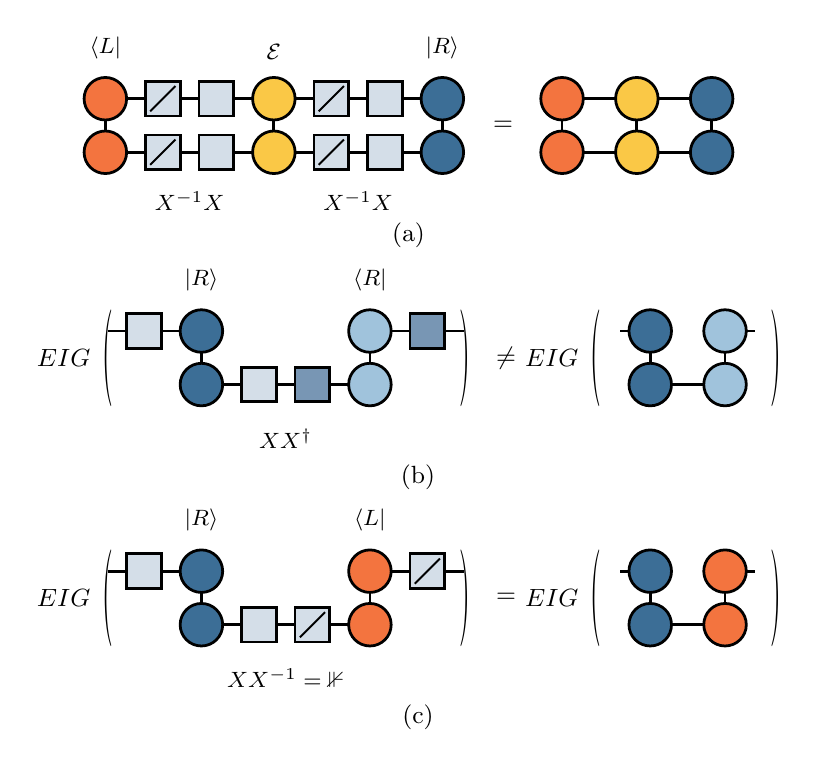
\begin{tikzpicture}[
    bond/.style={draw=black, line width=1.0pt},
    T/.style={circle, draw=black, line width=1.0pt, minimum size=5.4mm, inner sep=0pt},
    Xs/.style={rectangle, draw=black, line width=1.0pt, minimum size=4.4mm, inner sep=0pt},
    tag/.style={font=\small},
    idx/.style={font=\footnotesize},
  ]

  % gauge factors: plain X, X with a slash for the inverse, darker for the adjoint
  \newcommand{\gX}[2]{\node[Xs, fill=tnX] at (#1,#2) {};}
  \newcommand{\gXi}[2]{\node[Xs, fill=tnX] at (#1,#2) {};
    \draw[black, line width=0.7pt] ({#1-0.16},{#2-0.16}) -- ({#1+0.16},{#2+0.16});}
  \newcommand{\gXd}[2]{\node[Xs, fill=tnXd] at (#1,#2) {};}

  % a two-site column
  \newcommand{\col}[2]{\draw[bond] (#1,\HA) -- (#1,-\HA);
    \node[T, fill=#2] at (#1,\HA) {}; \node[T, fill=#2] at (#1,-\HA) {};}

  %% ================= (a) the insertion is free =================
  \begin{scope}[xshift=0.53cm, yshift=2.95cm]
    \foreach \y in {\HA,-\HA} { \draw[bond] (0,\y) -- (4.28,\y); }
    \foreach \y in {\HA,-\HA} { \gXi{0.73}{\y} \gX{1.41}{\y} \gXi{2.87}{\y} \gX{3.55}{\y} }
    \col{0}{tnL} \col{2.14}{tnE} \col{4.28}{tnR}
    \node[idx, anchor=south] at (0,0.72)    {$\bra{L}$};
    \node[idx, anchor=south] at (2.14,0.72) {$\mathcal{E}$};
    \node[idx, anchor=south] at (4.28,0.72) {$\ket{R}$};
    \node[idx, anchor=north] at (1.07,-0.72) {$X^{-1}X$};
    \node[idx, anchor=north] at (3.21,-0.72) {$X^{-1}X$};

    % the factors cancel pairwise, so the contraction is the ungauged one
    \node[tag] at (5.05,0) {$=$};
    \foreach \y in {\HA,-\HA} { \draw[bond] (5.80,\y) -- (7.70,\y); }
    \col{5.80}{tnL} \col{6.75}{tnE} \col{7.70}{tnR}

    \node[tag] at (3.85,-1.40) {(a)};
  \end{scope}

  % the two candidate objects. #1 xshift, #2 right fill, #3 partner of X on the contracted bond,
  % #4 the factor left on the right-hand open index. The gauge sits on every bond of the network,
  % so the open indices carry one factor each and the contracted bond carries both.
  \newcommand{\obj}[4]{%
    \begin{scope}[xshift=#1]
      \draw[bond] (-1.19,\HA) -- (0,\HA);             % open indices on the upper site
      \draw[bond] (2.14,\HA) -- (3.33,\HA);
      \gX{-0.73}{\HA} #4{2.87}{\HA}
      \draw[bond] (0,-\HA) -- (2.14,-\HA);            % the lower site is contracted
      \gX{0.73}{-\HA} #3{1.41}{-\HA}
      \col{0}{tnR} \col{2.14}{#2}
    \end{scope}}
  \newcommand{\objplain}[2]{%
    \begin{scope}[xshift=#1]
      \draw[bond] (-\ST,\HA) -- (0,\HA);
      \draw[bond] (0.95,\HA) -- ({0.95+\ST},\HA);
      \draw[bond] (0,-\HA) -- (0.95,-\HA);
      \col{0}{tnR} \col{0.95}{#2}
    \end{scope}}

  %% ================= (b) the RDM: the factors meet as X X^dagger =================
  \node[tag] at (0,0) {$EIG$};
  \node at (0.56,0) {\bigpar{(}};
  \obj{1.75cm}{tnRl}{\gXd}{\gXd}
  \node[idx, anchor=north] at (2.82,-0.78) {$X X^{\dagger}$};
  \node[idx, anchor=south] at (1.75,0.72) {$\ket{R}$};
  \node[idx, anchor=south] at (3.89,0.72) {$\bra{R}$};
  \node at (5.10,0) {\bigpar{)}};
  \node[tag] at (5.62,0) {$\neq$};
  \node[tag] at (6.20,0) {$EIG$};
  \node at (6.76,0) {\bigpar{(}};
  \objplain{7.45cm}{tnRl}
  \node at (9.05,0) {\bigpar{)}};
  \node[tag] at (4.5,-1.52) {(b)};

  %% ================= (c) the RTM: they meet as X X^{-1} =================
  \begin{scope}[yshift=-3.05cm]
    \node[tag] at (0,0) {$EIG$};
    \node at (0.56,0) {\bigpar{(}};
    \obj{1.75cm}{tnL}{\gXi}{\gXi}
    \node[idx, anchor=north] at (2.82,-0.78) {$X X^{-1}=\mathbb{1}$};
    \node[idx, anchor=south] at (1.75,0.72) {$\ket{R}$};
    \node[idx, anchor=south] at (3.89,0.72) {$\bra{L}$};
    \node at (5.10,0) {\bigpar{)}};
    \node[tag] at (5.62,0) {$=$};
    \node[tag] at (6.20,0) {$EIG$};
    \node at (6.76,0) {\bigpar{(}};
    \objplain{7.45cm}{tnL}
    \node at (9.05,0) {\bigpar{)}};
    \node[tag] at (4.5,-1.52) {(c)};
  \end{scope}

\end{tikzpicture}
\end{document}
.
\documentclass[tikz,border=3pt]{standalone}
\usepackage{amsmath,amssymb,braket,graphicx,bbold}
\usetikzlibrary{arrows.meta}

\definecolor{tnL}{RGB}{243,116,63}
\definecolor{tnR}{RGB}{60,110,150}
\definecolor{tnRl}{RGB}{160,195,220}
\definecolor{tnE}{RGB}{250,200,70}
\definecolor{tnX}{RGB}{212,222,232}
\definecolor{tnXd}{RGB}{120,150,180}

\newcommand{\HA}{0.34}
\newcommand{\ST}{0.38}
\newcommand{\bigpar}[1]{\scalebox{1.0}[3.5]{$#1$}}

\begin{document}
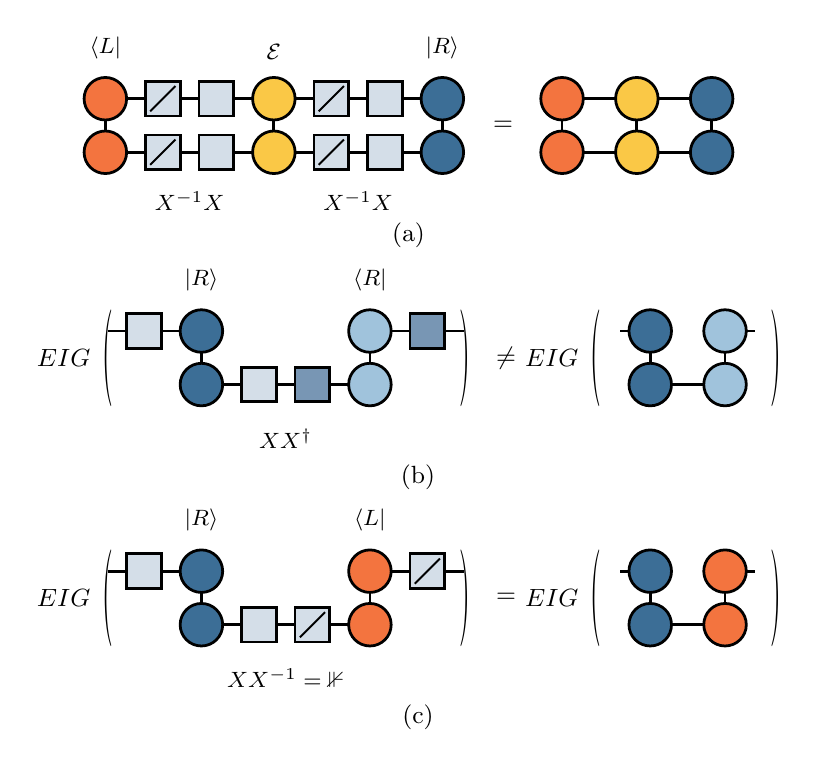
\begin{tikzpicture}[
    bond/.style={draw=black, line width=1.0pt},
    T/.style={circle, draw=black, line width=1.0pt, minimum size=5.4mm, inner sep=0pt},
    Xs/.style={rectangle, draw=black, line width=1.0pt, minimum size=4.4mm, inner sep=0pt},
    tag/.style={font=\small},
    idx/.style={font=\footnotesize},
  ]

  % gauge factors: plain X, X with a slash for the inverse, darker for the adjoint
  \newcommand{\gX}[2]{\node[Xs, fill=tnX] at (#1,#2) {};}
  \newcommand{\gXi}[2]{\node[Xs, fill=tnX] at (#1,#2) {};
    \draw[black, line width=0.7pt] ({#1-0.16},{#2-0.16}) -- ({#1+0.16},{#2+0.16});}
  \newcommand{\gXd}[2]{\node[Xs, fill=tnXd] at (#1,#2) {};}

  % a two-site column
  \newcommand{\col}[2]{\draw[bond] (#1,\HA) -- (#1,-\HA);
    \node[T, fill=#2] at (#1,\HA) {}; \node[T, fill=#2] at (#1,-\HA) {};}

  %% ================= (a) the insertion is free =================
  \begin{scope}[xshift=0.53cm, yshift=2.95cm]
    \foreach \y in {\HA,-\HA} { \draw[bond] (0,\y) -- (4.28,\y); }
    \foreach \y in {\HA,-\HA} { \gXi{0.73}{\y} \gX{1.41}{\y} \gXi{2.87}{\y} \gX{3.55}{\y} }
    \col{0}{tnL} \col{2.14}{tnE} \col{4.28}{tnR}
    \node[idx, anchor=south] at (0,0.72)    {$\bra{L}$};
    \node[idx, anchor=south] at (2.14,0.72) {$\mathcal{E}$};
    \node[idx, anchor=south] at (4.28,0.72) {$\ket{R}$};
    \node[idx, anchor=north] at (1.07,-0.72) {$X^{-1}X$};
    \node[idx, anchor=north] at (3.21,-0.72) {$X^{-1}X$};

    % the factors cancel pairwise, so the contraction is the ungauged one
    \node[tag] at (5.05,0) {$=$};
    \foreach \y in {\HA,-\HA} { \draw[bond] (5.80,\y) -- (7.70,\y); }
    \col{5.80}{tnL} \col{6.75}{tnE} \col{7.70}{tnR}

    \node[tag] at (3.85,-1.40) {(a)};
  \end{scope}

  % the two candidate objects. #1 xshift, #2 right fill, #3 partner of X on the contracted bond,
  % #4 the factor left on the right-hand open index. The gauge sits on every bond of the network,
  % so the open indices carry one factor each and the contracted bond carries both.
  \newcommand{\obj}[4]{%
    \begin{scope}[xshift=#1]
      \draw[bond] (-1.19,\HA) -- (0,\HA);             % open indices on the upper site
      \draw[bond] (2.14,\HA) -- (3.33,\HA);
      \gX{-0.73}{\HA} #4{2.87}{\HA}
      \draw[bond] (0,-\HA) -- (2.14,-\HA);            % the lower site is contracted
      \gX{0.73}{-\HA} #3{1.41}{-\HA}
      \col{0}{tnR} \col{2.14}{#2}
    \end{scope}}
  \newcommand{\objplain}[2]{%
    \begin{scope}[xshift=#1]
      \draw[bond] (-\ST,\HA) -- (0,\HA);
      \draw[bond] (0.95,\HA) -- ({0.95+\ST},\HA);
      \draw[bond] (0,-\HA) -- (0.95,-\HA);
      \col{0}{tnR} \col{0.95}{#2}
    \end{scope}}

  %% ================= (b) the RDM: the factors meet as X X^dagger =================
  \node[tag] at (0,0) {$EIG$};
  \node at (0.56,0) {\bigpar{(}};
  \obj{1.75cm}{tnRl}{\gXd}{\gXd}
  \node[idx, anchor=north] at (2.82,-0.78) {$X X^{\dagger}$};
  \node[idx, anchor=south] at (1.75,0.72) {$\ket{R}$};
  \node[idx, anchor=south] at (3.89,0.72) {$\bra{R}$};
  \node at (5.10,0) {\bigpar{)}};
  \node[tag] at (5.62,0) {$\neq$};
  \node[tag] at (6.20,0) {$EIG$};
  \node at (6.76,0) {\bigpar{(}};
  \objplain{7.45cm}{tnRl}
  \node at (9.05,0) {\bigpar{)}};
  \node[tag] at (4.5,-1.52) {(b)};

  %% ================= (c) the RTM: they meet as X X^{-1} =================
  \begin{scope}[yshift=-3.05cm]
    \node[tag] at (0,0) {$EIG$};
    \node at (0.56,0) {\bigpar{(}};
    \obj{1.75cm}{tnL}{\gXi}{\gXi}
    \node[idx, anchor=north] at (2.82,-0.78) {$X X^{-1}=\mathbb{1}$};
    \node[idx, anchor=south] at (1.75,0.72) {$\ket{R}$};
    \node[idx, anchor=south] at (3.89,0.72) {$\bra{L}$};
    \node at (5.10,0) {\bigpar{)}};
    \node[tag] at (5.62,0) {$=$};
    \node[tag] at (6.20,0) {$EIG$};
    \node at (6.76,0) {\bigpar{(}};
    \objplain{7.45cm}{tnL}
    \node at (9.05,0) {\bigpar{)}};
    \node[tag] at (4.5,-1.52) {(c)};
  \end{scope}

\end{tikzpicture}
\end{document}
.
\documentclass[tikz,border=3pt]{standalone}
\usepackage{amsmath,amssymb,braket,graphicx,bbold}
\usetikzlibrary{arrows.meta}

\definecolor{tnL}{RGB}{243,116,63}
\definecolor{tnR}{RGB}{60,110,150}
\definecolor{tnRl}{RGB}{160,195,220}
\definecolor{tnE}{RGB}{250,200,70}
\definecolor{tnX}{RGB}{212,222,232}
\definecolor{tnXd}{RGB}{120,150,180}

\newcommand{\HA}{0.34}
\newcommand{\ST}{0.38}
\newcommand{\bigpar}[1]{\scalebox{1.0}[3.5]{$#1$}}

\begin{document}
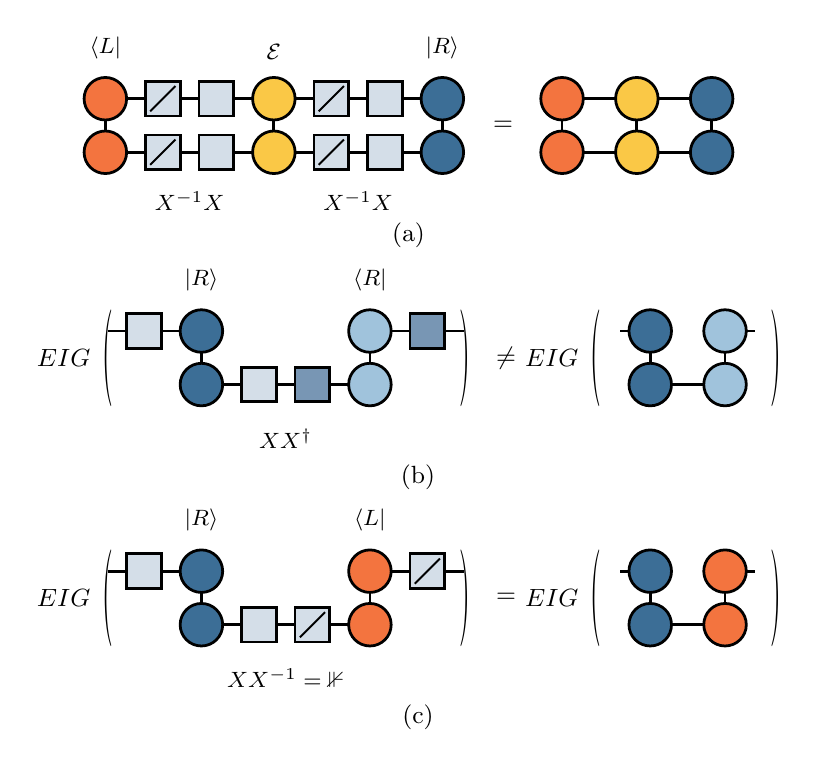
\begin{tikzpicture}[
    bond/.style={draw=black, line width=1.0pt},
    T/.style={circle, draw=black, line width=1.0pt, minimum size=5.4mm, inner sep=0pt},
    Xs/.style={rectangle, draw=black, line width=1.0pt, minimum size=4.4mm, inner sep=0pt},
    tag/.style={font=\small},
    idx/.style={font=\footnotesize},
  ]

  % gauge factors: plain X, X with a slash for the inverse, darker for the adjoint
  \newcommand{\gX}[2]{\node[Xs, fill=tnX] at (#1,#2) {};}
  \newcommand{\gXi}[2]{\node[Xs, fill=tnX] at (#1,#2) {};
    \draw[black, line width=0.7pt] ({#1-0.16},{#2-0.16}) -- ({#1+0.16},{#2+0.16});}
  \newcommand{\gXd}[2]{\node[Xs, fill=tnXd] at (#1,#2) {};}

  % a two-site column
  \newcommand{\col}[2]{\draw[bond] (#1,\HA) -- (#1,-\HA);
    \node[T, fill=#2] at (#1,\HA) {}; \node[T, fill=#2] at (#1,-\HA) {};}

  %% ================= (a) the insertion is free =================
  \begin{scope}[xshift=0.53cm, yshift=2.95cm]
    \foreach \y in {\HA,-\HA} { \draw[bond] (0,\y) -- (4.28,\y); }
    \foreach \y in {\HA,-\HA} { \gXi{0.73}{\y} \gX{1.41}{\y} \gXi{2.87}{\y} \gX{3.55}{\y} }
    \col{0}{tnL} \col{2.14}{tnE} \col{4.28}{tnR}
    \node[idx, anchor=south] at (0,0.72)    {$\bra{L}$};
    \node[idx, anchor=south] at (2.14,0.72) {$\mathcal{E}$};
    \node[idx, anchor=south] at (4.28,0.72) {$\ket{R}$};
    \node[idx, anchor=north] at (1.07,-0.72) {$X^{-1}X$};
    \node[idx, anchor=north] at (3.21,-0.72) {$X^{-1}X$};

    % the factors cancel pairwise, so the contraction is the ungauged one
    \node[tag] at (5.05,0) {$=$};
    \foreach \y in {\HA,-\HA} { \draw[bond] (5.80,\y) -- (7.70,\y); }
    \col{5.80}{tnL} \col{6.75}{tnE} \col{7.70}{tnR}

    \node[tag] at (3.85,-1.40) {(a)};
  \end{scope}

  % the two candidate objects. #1 xshift, #2 right fill, #3 partner of X on the contracted bond,
  % #4 the factor left on the right-hand open index. The gauge sits on every bond of the network,
  % so the open indices carry one factor each and the contracted bond carries both.
  \newcommand{\obj}[4]{%
    \begin{scope}[xshift=#1]
      \draw[bond] (-1.19,\HA) -- (0,\HA);             % open indices on the upper site
      \draw[bond] (2.14,\HA) -- (3.33,\HA);
      \gX{-0.73}{\HA} #4{2.87}{\HA}
      \draw[bond] (0,-\HA) -- (2.14,-\HA);            % the lower site is contracted
      \gX{0.73}{-\HA} #3{1.41}{-\HA}
      \col{0}{tnR} \col{2.14}{#2}
    \end{scope}}
  \newcommand{\objplain}[2]{%
    \begin{scope}[xshift=#1]
      \draw[bond] (-\ST,\HA) -- (0,\HA);
      \draw[bond] (0.95,\HA) -- ({0.95+\ST},\HA);
      \draw[bond] (0,-\HA) -- (0.95,-\HA);
      \col{0}{tnR} \col{0.95}{#2}
    \end{scope}}

  %% ================= (b) the RDM: the factors meet as X X^dagger =================
  \node[tag] at (0,0) {$EIG$};
  \node at (0.56,0) {\bigpar{(}};
  \obj{1.75cm}{tnRl}{\gXd}{\gXd}
  \node[idx, anchor=north] at (2.82,-0.78) {$X X^{\dagger}$};
  \node[idx, anchor=south] at (1.75,0.72) {$\ket{R}$};
  \node[idx, anchor=south] at (3.89,0.72) {$\bra{R}$};
  \node at (5.10,0) {\bigpar{)}};
  \node[tag] at (5.62,0) {$\neq$};
  \node[tag] at (6.20,0) {$EIG$};
  \node at (6.76,0) {\bigpar{(}};
  \objplain{7.45cm}{tnRl}
  \node at (9.05,0) {\bigpar{)}};
  \node[tag] at (4.5,-1.52) {(b)};

  %% ================= (c) the RTM: they meet as X X^{-1} =================
  \begin{scope}[yshift=-3.05cm]
    \node[tag] at (0,0) {$EIG$};
    \node at (0.56,0) {\bigpar{(}};
    \obj{1.75cm}{tnL}{\gXi}{\gXi}
    \node[idx, anchor=north] at (2.82,-0.78) {$X X^{-1}=\mathbb{1}$};
    \node[idx, anchor=south] at (1.75,0.72) {$\ket{R}$};
    \node[idx, anchor=south] at (3.89,0.72) {$\bra{L}$};
    \node at (5.10,0) {\bigpar{)}};
    \node[tag] at (5.62,0) {$=$};
    \node[tag] at (6.20,0) {$EIG$};
    \node at (6.76,0) {\bigpar{(}};
    \objplain{7.45cm}{tnL}
    \node at (9.05,0) {\bigpar{)}};
    \node[tag] at (4.5,-1.52) {(c)};
  \end{scope}

\end{tikzpicture}
\end{document}
.
\documentclass[tikz,border=3pt]{standalone}
\usepackage{amsmath,amssymb,braket,graphicx,bbold}
\usetikzlibrary{arrows.meta}

\definecolor{tnL}{RGB}{243,116,63}
\definecolor{tnR}{RGB}{60,110,150}
\definecolor{tnRl}{RGB}{160,195,220}
\definecolor{tnE}{RGB}{250,200,70}
\definecolor{tnX}{RGB}{212,222,232}
\definecolor{tnXd}{RGB}{120,150,180}

\newcommand{\HA}{0.34}
\newcommand{\ST}{0.38}
\newcommand{\bigpar}[1]{\scalebox{1.0}[3.5]{$#1$}}

\begin{document}
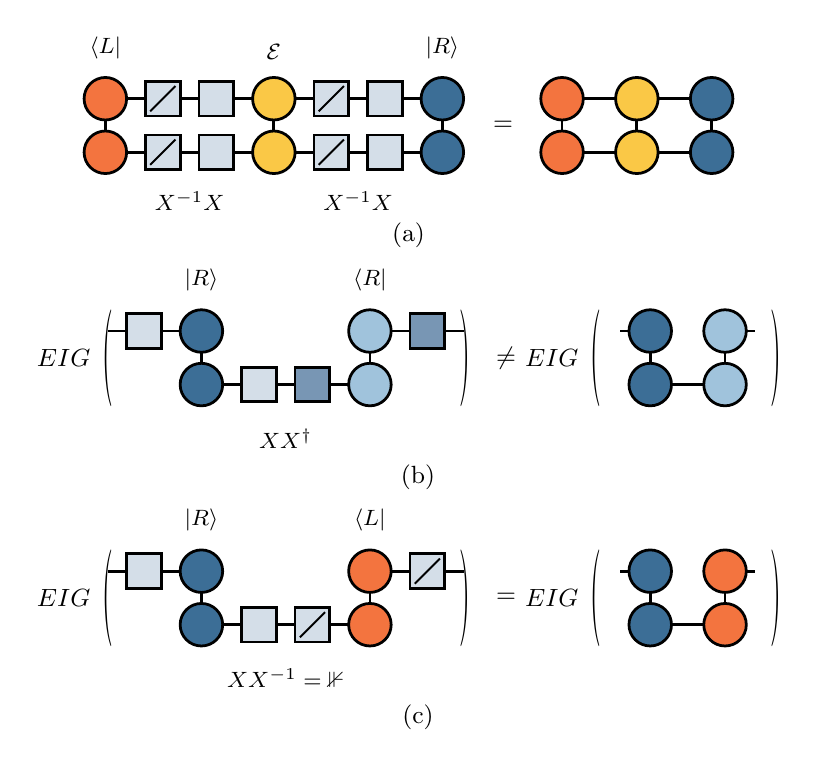
\begin{tikzpicture}[
    bond/.style={draw=black, line width=1.0pt},
    T/.style={circle, draw=black, line width=1.0pt, minimum size=5.4mm, inner sep=0pt},
    Xs/.style={rectangle, draw=black, line width=1.0pt, minimum size=4.4mm, inner sep=0pt},
    tag/.style={font=\small},
    idx/.style={font=\footnotesize},
  ]

  % gauge factors: plain X, X with a slash for the inverse, darker for the adjoint
  \newcommand{\gX}[2]{\node[Xs, fill=tnX] at (#1,#2) {};}
  \newcommand{\gXi}[2]{\node[Xs, fill=tnX] at (#1,#2) {};
    \draw[black, line width=0.7pt] ({#1-0.16},{#2-0.16}) -- ({#1+0.16},{#2+0.16});}
  \newcommand{\gXd}[2]{\node[Xs, fill=tnXd] at (#1,#2) {};}

  % a two-site column
  \newcommand{\col}[2]{\draw[bond] (#1,\HA) -- (#1,-\HA);
    \node[T, fill=#2] at (#1,\HA) {}; \node[T, fill=#2] at (#1,-\HA) {};}

  %% ================= (a) the insertion is free =================
  \begin{scope}[xshift=0.53cm, yshift=2.95cm]
    \foreach \y in {\HA,-\HA} { \draw[bond] (0,\y) -- (4.28,\y); }
    \foreach \y in {\HA,-\HA} { \gXi{0.73}{\y} \gX{1.41}{\y} \gXi{2.87}{\y} \gX{3.55}{\y} }
    \col{0}{tnL} \col{2.14}{tnE} \col{4.28}{tnR}
    \node[idx, anchor=south] at (0,0.72)    {$\bra{L}$};
    \node[idx, anchor=south] at (2.14,0.72) {$\mathcal{E}$};
    \node[idx, anchor=south] at (4.28,0.72) {$\ket{R}$};
    \node[idx, anchor=north] at (1.07,-0.72) {$X^{-1}X$};
    \node[idx, anchor=north] at (3.21,-0.72) {$X^{-1}X$};

    % the factors cancel pairwise, so the contraction is the ungauged one
    \node[tag] at (5.05,0) {$=$};
    \foreach \y in {\HA,-\HA} { \draw[bond] (5.80,\y) -- (7.70,\y); }
    \col{5.80}{tnL} \col{6.75}{tnE} \col{7.70}{tnR}

    \node[tag] at (3.85,-1.40) {(a)};
  \end{scope}

  % the two candidate objects. #1 xshift, #2 right fill, #3 partner of X on the contracted bond,
  % #4 the factor left on the right-hand open index. The gauge sits on every bond of the network,
  % so the open indices carry one factor each and the contracted bond carries both.
  \newcommand{\obj}[4]{%
    \begin{scope}[xshift=#1]
      \draw[bond] (-1.19,\HA) -- (0,\HA);             % open indices on the upper site
      \draw[bond] (2.14,\HA) -- (3.33,\HA);
      \gX{-0.73}{\HA} #4{2.87}{\HA}
      \draw[bond] (0,-\HA) -- (2.14,-\HA);            % the lower site is contracted
      \gX{0.73}{-\HA} #3{1.41}{-\HA}
      \col{0}{tnR} \col{2.14}{#2}
    \end{scope}}
  \newcommand{\objplain}[2]{%
    \begin{scope}[xshift=#1]
      \draw[bond] (-\ST,\HA) -- (0,\HA);
      \draw[bond] (0.95,\HA) -- ({0.95+\ST},\HA);
      \draw[bond] (0,-\HA) -- (0.95,-\HA);
      \col{0}{tnR} \col{0.95}{#2}
    \end{scope}}

  %% ================= (b) the RDM: the factors meet as X X^dagger =================
  \node[tag] at (0,0) {$EIG$};
  \node at (0.56,0) {\bigpar{(}};
  \obj{1.75cm}{tnRl}{\gXd}{\gXd}
  \node[idx, anchor=north] at (2.82,-0.78) {$X X^{\dagger}$};
  \node[idx, anchor=south] at (1.75,0.72) {$\ket{R}$};
  \node[idx, anchor=south] at (3.89,0.72) {$\bra{R}$};
  \node at (5.10,0) {\bigpar{)}};
  \node[tag] at (5.62,0) {$\neq$};
  \node[tag] at (6.20,0) {$EIG$};
  \node at (6.76,0) {\bigpar{(}};
  \objplain{7.45cm}{tnRl}
  \node at (9.05,0) {\bigpar{)}};
  \node[tag] at (4.5,-1.52) {(b)};

  %% ================= (c) the RTM: they meet as X X^{-1} =================
  \begin{scope}[yshift=-3.05cm]
    \node[tag] at (0,0) {$EIG$};
    \node at (0.56,0) {\bigpar{(}};
    \obj{1.75cm}{tnL}{\gXi}{\gXi}
    \node[idx, anchor=north] at (2.82,-0.78) {$X X^{-1}=\mathbb{1}$};
    \node[idx, anchor=south] at (1.75,0.72) {$\ket{R}$};
    \node[idx, anchor=south] at (3.89,0.72) {$\bra{L}$};
    \node at (5.10,0) {\bigpar{)}};
    \node[tag] at (5.62,0) {$=$};
    \node[tag] at (6.20,0) {$EIG$};
    \node at (6.76,0) {\bigpar{(}};
    \objplain{7.45cm}{tnL}
    \node at (9.05,0) {\bigpar{)}};
    \node[tag] at (4.5,-1.52) {(c)};
  \end{scope}

\end{tikzpicture}
\end{document}
